% \PassOptionsToPackage{quiet}{fontspec}
\documentclass[12pt,a4paper,UTF8]{article}
\usepackage{thesis} % 格式控制
\setlength{\parindent}{2em} % 控制首行缩进  
\addtolength{\parskip}{3pt} % 控制段落距离  
\onehalfspacing % 1.5倍行距  
\graphicspath{{./figures/}} % 指定图片所在文件夹  

\usepackage{dirtree}
\classname{智能控制技术}  % 设置课程名称
\expname{HW04 神经网络辨识}
\makepagestyle{\printexpname}{\printclassname ~实验报告}

\begin{document}
\maketitlepage{\printexpname}{教7 304}{PhilFan}{19260817}{\today}{刘山} %封面页 

\maketoc    %目录页
\section{实验目的和要求}

如图所示二自由度机械臂模型(平面俯视图),$q_1$和$q_2$表示机械臂的两个关节角大小。

\begin{figure}[htbp]
    \centering
    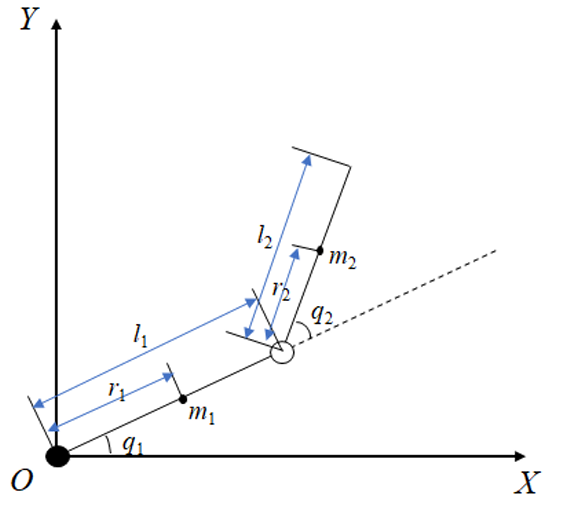
\includegraphics[width=0.3\textwidth]{figures/20241206103243.png}
    \caption{二自由度机械臂模型}
    \label{fig:robot-arm}
\end{figure}

图中,$m_i, l_i, r_i (i=1,2)$分别为两连杆的质量、连杆长度和质心到相应关节的距离。

两个连杆的转动惯量分别为$I_1$和$I_2$。该机械臂动力学方程表示为:

\begin{equation}
M(q)\ddot{q} + C(q, \dot{q})\dot{q} + G(q) = \tau 
\end{equation}

$M(q)$为惯性矩阵,$C(q, \dot{q})$为科氏力和向心力的结合矩阵,$G(q)$为重力势能矩阵。

$\tau$为驱动力矩的向量。式(1)可写为如下方式:

\begin{equation}
\begin{aligned}
m_{11}\ddot{q}_1 + m_{12}\ddot{q}_2 + c_{11}\dot{q}_1 + c_{12}\dot{q}_2 + g_1 &= \tau_1 \\
m_{21}\ddot{q}_1 + m_{22}\ddot{q}_2 + c_{21}\dot{q}_1 + c_{22}\dot{q}_2 + g_2 &= \tau_2
\end{aligned}
\end{equation}

$\tau_1$、$\tau_2$分别为关节1和关节2的驱动力矩。

定义以下参数:

\begin{equation}
\begin{aligned}
h_1 &= m_1r_1^2 + m_2l_2^2 + I_1 \\
h_2 &= m_2r_2^2 + I_2 \\
h_3 &= m_2l_1r_2 \\
h_4 &= m_1r_1 + m_2l_1 \\
h_5 &= m_2r_2
\end{aligned}
\end{equation}

则式(2)和式(3)中的参数可按如下计算:

\begin{equation}
\begin{aligned}
m_{11} &= h_1 + h_2 + 2h_3 \cos(q_2) \\
m_{12} = m_{21} &= h_2 + h_3 \cos(q_2) \\
m_{22} &= h_2 \\
c_{11} &= -h_3 \sin(q_2) \dot{q}_2 \\
c_{12} &= -h_3 \sin(q_2) (\dot{q}_1 + \dot{q}_2) \\
c_{21} &= h_3 \sin(q_2) \dot{q}_1\\
c_{22} &= 0 \\
g_1 &= h_4 g \cos(q_1) + h_5 g \cos(q_1 + q_2) \\
g_2 &= h_5 g \cos(q_1 + q_2) 
\end{aligned}
\end{equation}

式中,$g$为重力加速度$9.8m/s^2$。

假定系统参数如下表所示:

\begin{table}[htbp]
\centering
\begin{tabular}{|c|c|}
\hline
参数 & 数值 \\
\hline
$h_1$ & 0.0308 \\
$h_2$ & 0.0106 \\
$h_3$ & 0.0095 \\
$h_4$ & 0.2086 \\
$h_5$ & 0.0631 \\
\hline
\end{tabular}
\caption{系统参数表}
\label{tab:parameters}
\end{table}


\begin{problem}
请设计神经网络辨识方案,对该系统进行辨识(系统输入为$\tau_1, \tau_2$,输出为$q_1, q_2$)

参考步骤:
\begin{enumerate}
    \item 利用已知系统得到辨识所需的输入输出数据;
    \item 通过步骤1得到的数据来训练神经网络;
    \item 对比原系统与神经网络辨识得到的系统是否一致。(给两个系统同样的输入,观察输出是否相同)(可以利用Matlab中的相关工具箱进行仿真)
\end{enumerate}
    
\end{problem}




\clearpage % 换页
\section{Deep Learning Toolbox 学习}

首先我根据助教的视频,和b站上的视频,学习了神经网络工具箱的基本用法,具体用到的数据和代码放到\texttt{learn\_toolbox}文件夹中

之后下一届如果可以的话,希望每次教程都可以有一个小例子或小数据集用来实操,我也把这次我自学用到的数据和代码放到\texttt{learn\_toolbox}文件夹中

当然,使用工具箱自带的一些数据集也是可以的。

\begin{lstlisting}[language=Matlab,caption=打开神经网络工具箱]
nftool
\end{lstlisting}

\begin{itemize}
    \item 选择导入数据集
    \item 正确选择是行还是列
    \item 选择训练集的比例;隐藏层的个数(5or10)
    \item 选择训练方法:一般选择第一个方法;第二个方法和遗传算法一起用;第三个方法比较慢
\end{itemize}

\textbf{提示:} validation test 表示的是泛化性能,如果连续6个epoch都上不去,就停止训练

图像查看:一般看回归的图(第四个),如果都上了0.9差不多就可以了

\begin{figure}[htbp] \centering 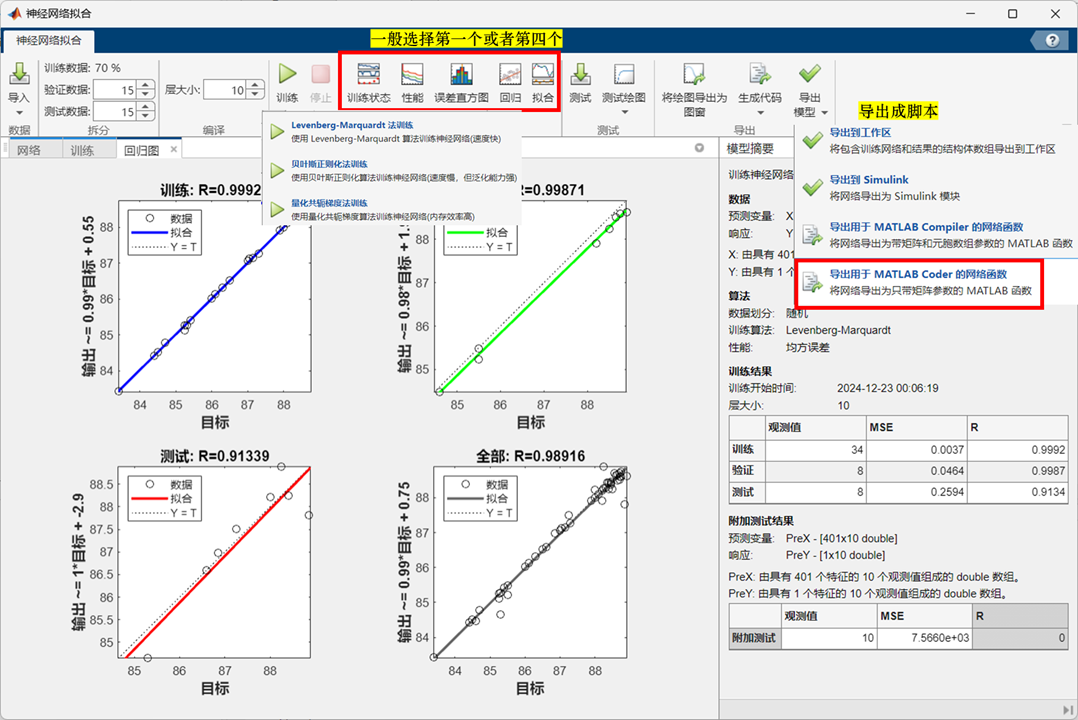
\includegraphics[width=0.7\textwidth]{figures/2024-12-24-00-27-14.png} \caption{神经网络工具箱的使用} \label{  }\end{figure}

\subsection{模型保存}
\begin{lstlisting}[language=Matlab,caption=保存模型]
save('filename.mat')  % 保存所有变量
save('filename.mat', 'var1', 'var2')  % 只保存指定变量
\end{lstlisting}

\begin{lstlisting}[language=Matlab,caption=从.mat文件中导入数据]
load('data.mat');
\end{lstlisting}

\subsection{模型预测}

\begin{lstlisting}[language=Matlab,caption=方法1:使用sim函数]
PreY = zeros(10,1);
for i = 1:10
    PreY(i,1) = sim(net,PreX(i,:)');
    % sim函数第二个参数列数等于输入向量的个数
end
disp(PreY);
\end{lstlisting}

\begin{lstlisting}[language=Matlab,caption=方法2:使用生成的函数]
myNeuralNetworkFunction(X) % 这里需要把后两个参数去掉
\end{lstlisting}
 
\subsection{多输入多输出}

多输入多输出也是一样的操作,唯一值得注意的地方就是在训练之前需要将行还是列选择正确(特征or样本)

\subsection{使用脚本替代ui操作}

\begin{lstlisting}[language=Matlab,caption=使用脚本替代ui操作,并且函数化]
function train()
    dataFile = 'data.mat';
    load(dataFile);  % 从文件导入数据
    x = features';  % 转置为符合网络输入格式
    t = labels';  % 转置为符合网络目标格式

    % 选择训练函数
    trainFcn = 'trainlm';  % Levenberg-Marquardt 反向传播

    % 创建拟合网络
    hiddenLayerSize = 15;
    net = fitnet(hiddenLayerSize, trainFcn);

    % 输入输出的预处理函数
    net.input.processFcns = {'removeconstantrows', 'mapminmax'};
    net.output.processFcns = {'removeconstantrows', 'mapminmax'};

    % 设置数据的划分方式
    net.divideFcn = 'dividerand';  % 随机划分数据
    net.divideMode = 'sample';  % 划分所有样本
    net.divideParam.trainRatio = 70/100;
    net.divideParam.valRatio = 15/100;
    net.divideParam.testRatio = 15/100;

    % 选择性能函数
    net.performFcn = 'mse';  % 均方误差

    % 选择绘图函数
    net.plotFcns = {'plotperform', 'plottrainstate', 'ploterrhist', ...
        'plotregression', 'plotfit'};

    % 训练网络
    [net, tr] = train(net, x, t);

    % 测试网络
    y = net(x);
    e = gsubtract(t, y);
    performance = perform(net, t, y);

    % 重新计算训练、验证和测试性能
    trainTargets = t .* tr.trainMask{1};
    valTargets = t .* tr.valMask{1};
    testTargets = t .* tr.testMask{1};
    trainPerformance = perform(net, trainTargets, y);
    valPerformance = perform(net, valTargets, y);
    testPerformance = perform(net, testTargets, y);

    figure, plotperform(tr);% 绘制并保存训练性能图
%     figure, plottrainstate(tr);% 绘制并保存训练状态图
%     figure, ploterrhist(e);% 绘制并保存误差直方图
    figure, plotregression(t, y)
%     figure, plotfit(net, x, t);% 绘制并保存拟合图

    % 保存模型
%     modelFile = ['model_level' num2str(level) '.mat'];
%     save(modelFile, 'net');  % 保存神经网络模型
    % 生成simulink模型
    gensim(net);
    disp(['Model saved as ' modelFile]);
end
\end{lstlisting}


\section{问题分析}
\subsection{问题建模分析}

首先题目中明确这是一个多输入多输出的问题,系统输入为$\tau_1, \tau_2$,输出为$q_1, q_2$

那么第一个问题就是获取系统输入输出数据,这里我有两个思路,一个是使用s-funtion进行生成数据,另一种思路是使用python脚本直接生成数据,鉴于后续还需要使用s-funtion进行仿真,所以这里选择使用s-funtion进行生成数据


值得注意的是,我这里在使用s-funtion的时候,同步将数据记录在了全局变量当中,最后阶数的时候,通过一定的处理步骤,直接生成了二阶和三阶的训练数据的\texttt{.mat}文件,无需进行工作区导入变量等处理,简化了实验的步骤。




\subsection{神经网络的训练}

使用nftool进行训练,可以观察到四个R都大于0.9 效果还不错,生成simulink模型之后

将其复制进slx文件中进行仿真

这里我写的函数可以直接调用`train(2)`训练二阶模型,调用`train(3)`训练三阶模型
自动加载文件夹下的数据,并进行训练,训练完成之后,自动保存模型并生成图像和simulink模型


\begin{figure}[htbp] \centering 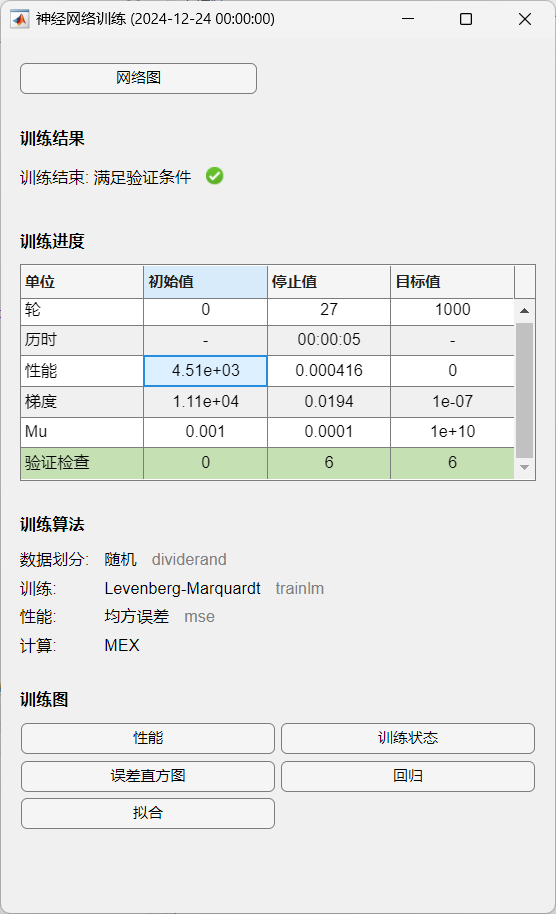
\includegraphics[width=0.3\textwidth]{figures/2024-12-24-00-01-06.png} \caption{  } \label{  }\end{figure}

\begin{figure}[htbp] \centering 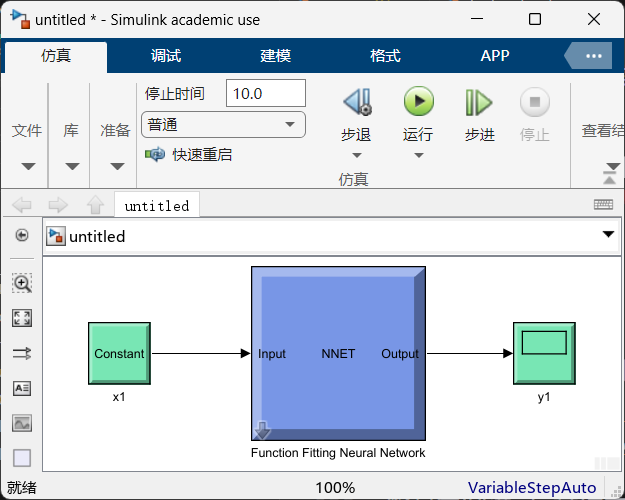
\includegraphics[width=0.4\textwidth]{figures/2024-12-24-00-01-14.png} \caption{生成的模型} \label{  }\end{figure}

\begin{figure}[htbp] \centering 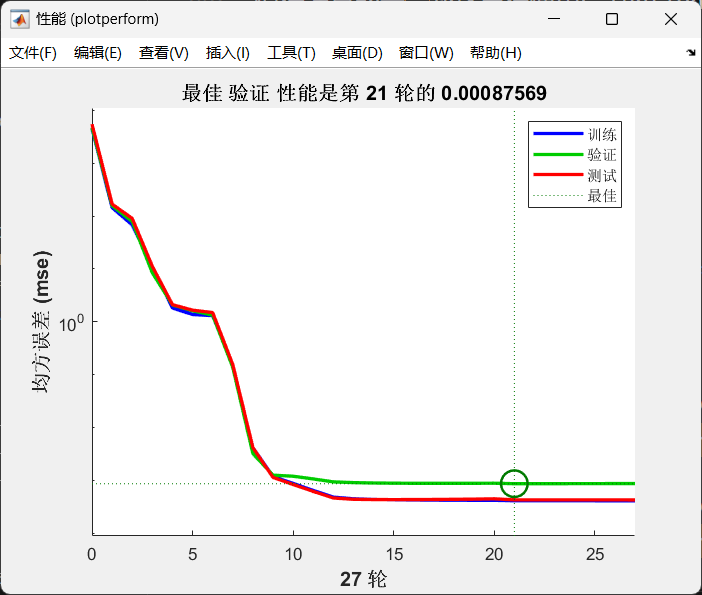
\includegraphics[width=0.4\textwidth]{figures/2024-12-24-00-01-25.png} \caption{训练图像} \label{  }\end{figure}

\begin{figure}[htbp] \centering 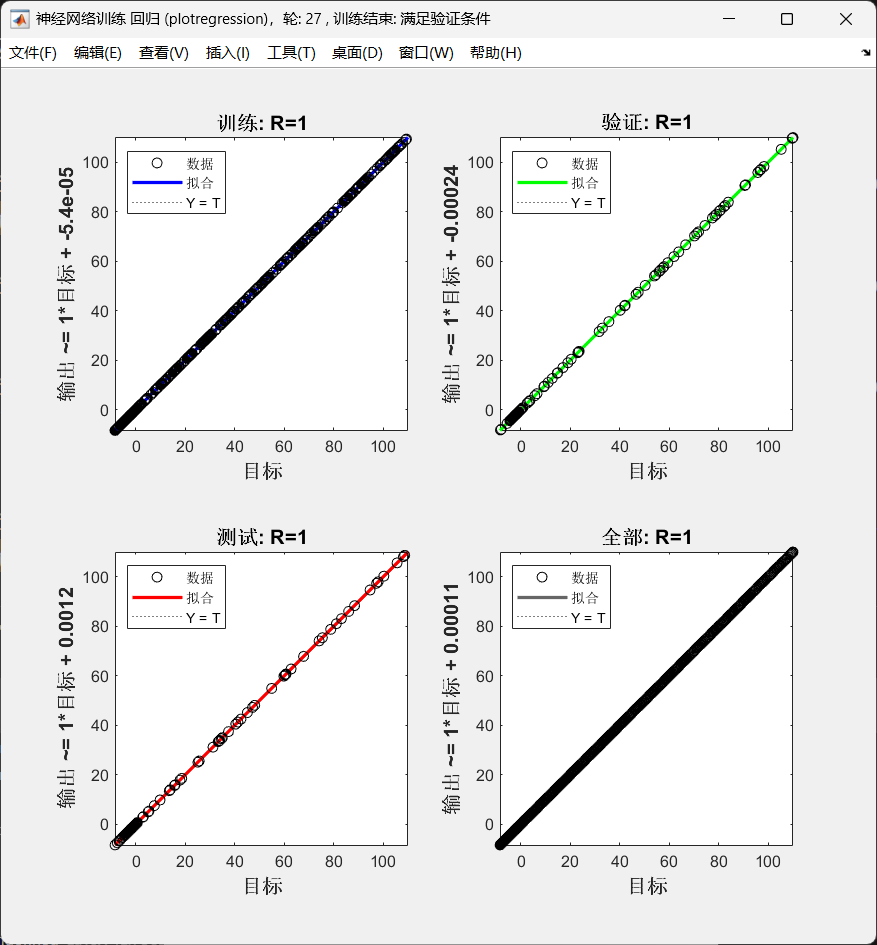
\includegraphics[width=0.4\textwidth]{figures/2024-12-24-00-01-58.png} \caption{回归图像} \label{  }\end{figure}


\subsection{神经网络保存}

\begin{figure}[htbp] \centering 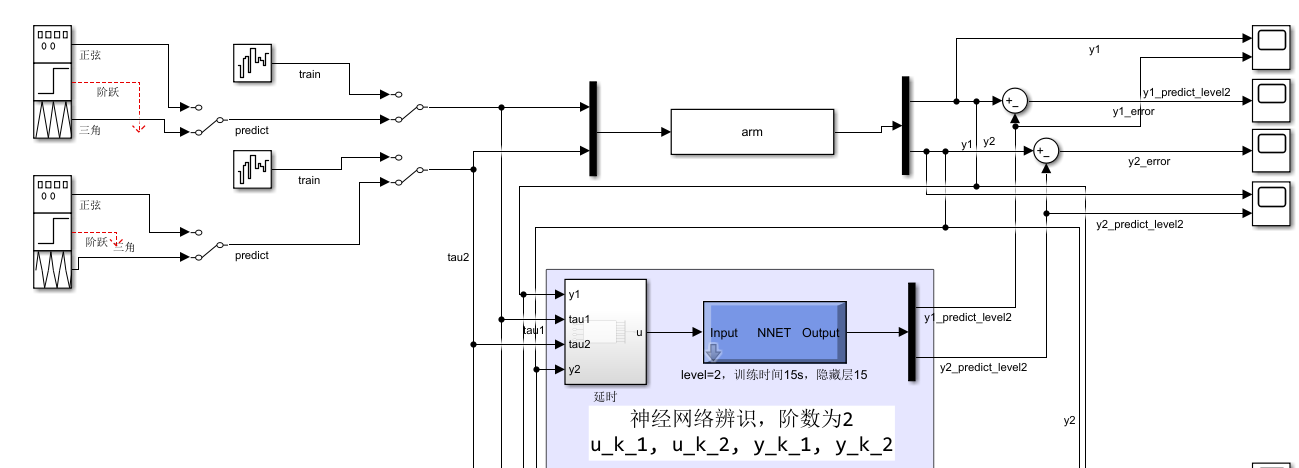
\includegraphics[width=0.7\textwidth]{figures/2024-12-23-23-58-06.png} \caption{搭好的模型如下} \label{  }\end{figure}

这里需要注意的是,串并联模型需要将$u_{k-1}, u_{k-2}$等作为输入,所以需要将这些变量作为输入端口添加到模型中

这里我将延时部分创建了子系统,这样看起来比较清爽一点。


\subsection{切换参数重新训练}

使用白噪声作为输入进行训练,使用正弦、阶跃、三角作为输入进行测试

这里我使用了单刀双掷开关,将输入端口和延时端口进行切换,从而实现不同输入的切换

这里为了验证不同初始情况下的模型效果,我测试了以下几个方面:

\begin{itemize}
    \item 二阶和三阶模型的效果对比
    \item 不同隐藏层数量(5,10,15)下的效果对比
    \item 不同白噪声输入幅值(0.1,0.5,1.0)下的效果对比
    \item 不同输入信号(正弦、阶跃、三角)下的效果对比
    \item 不同时间下(5s,15s,30s)下的效果对比
\end{itemize}


具体实现效果详见下一节


\clearpage
\section{实验结果表现与分析}
对于每一种训练出来的模型,我都使用正弦、阶跃、三角三种输入信号进行测试,并记录了不同输入信号下的效果对比


\begin{figure}[htbp] \centering 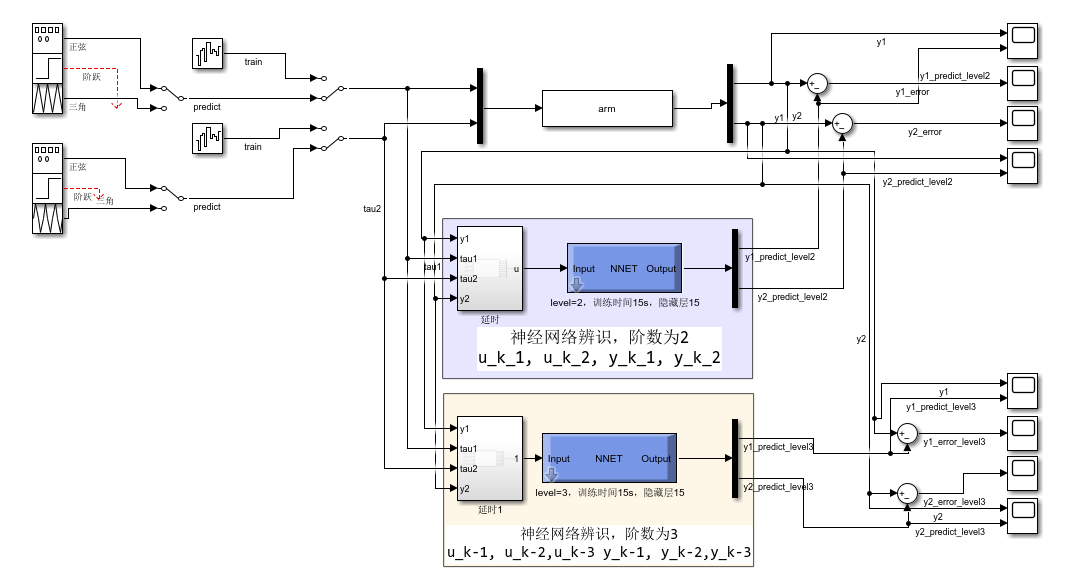
\includegraphics[width=0.7\textwidth]{figures/2024-12-24-00-21-09.png} \caption{训练的模型图片} \label{  }\end{figure}
\subsection{二阶和三阶模型的效果对比}
\begin{figure}[htbp] \centering 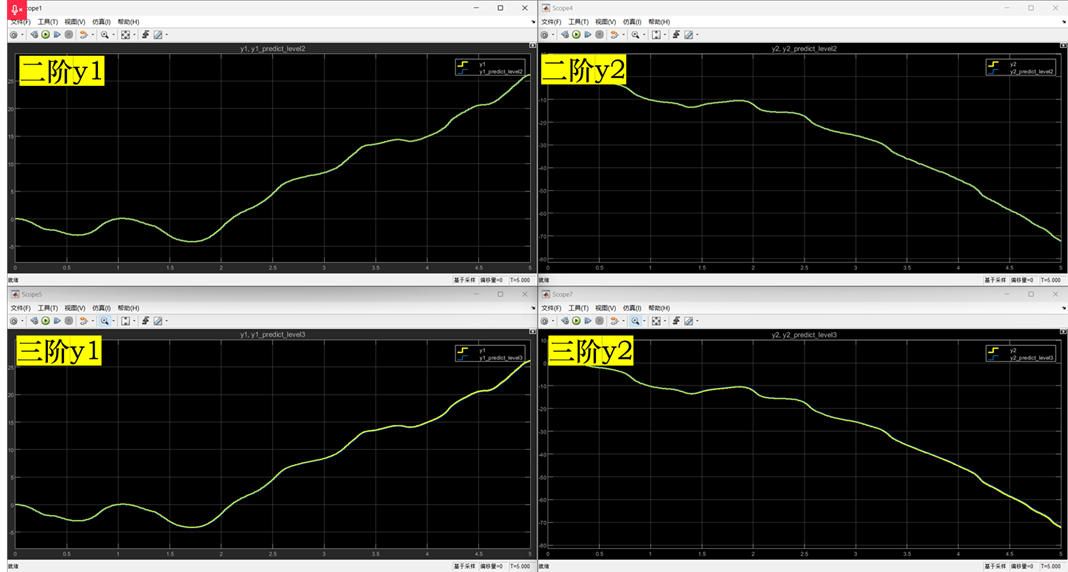
\includegraphics[width=0.7\textwidth]{figures/2024-12-24-00-24-40.png} \caption{正弦输入} \label{  }\end{figure}

\begin{figure}[htbp] \centering 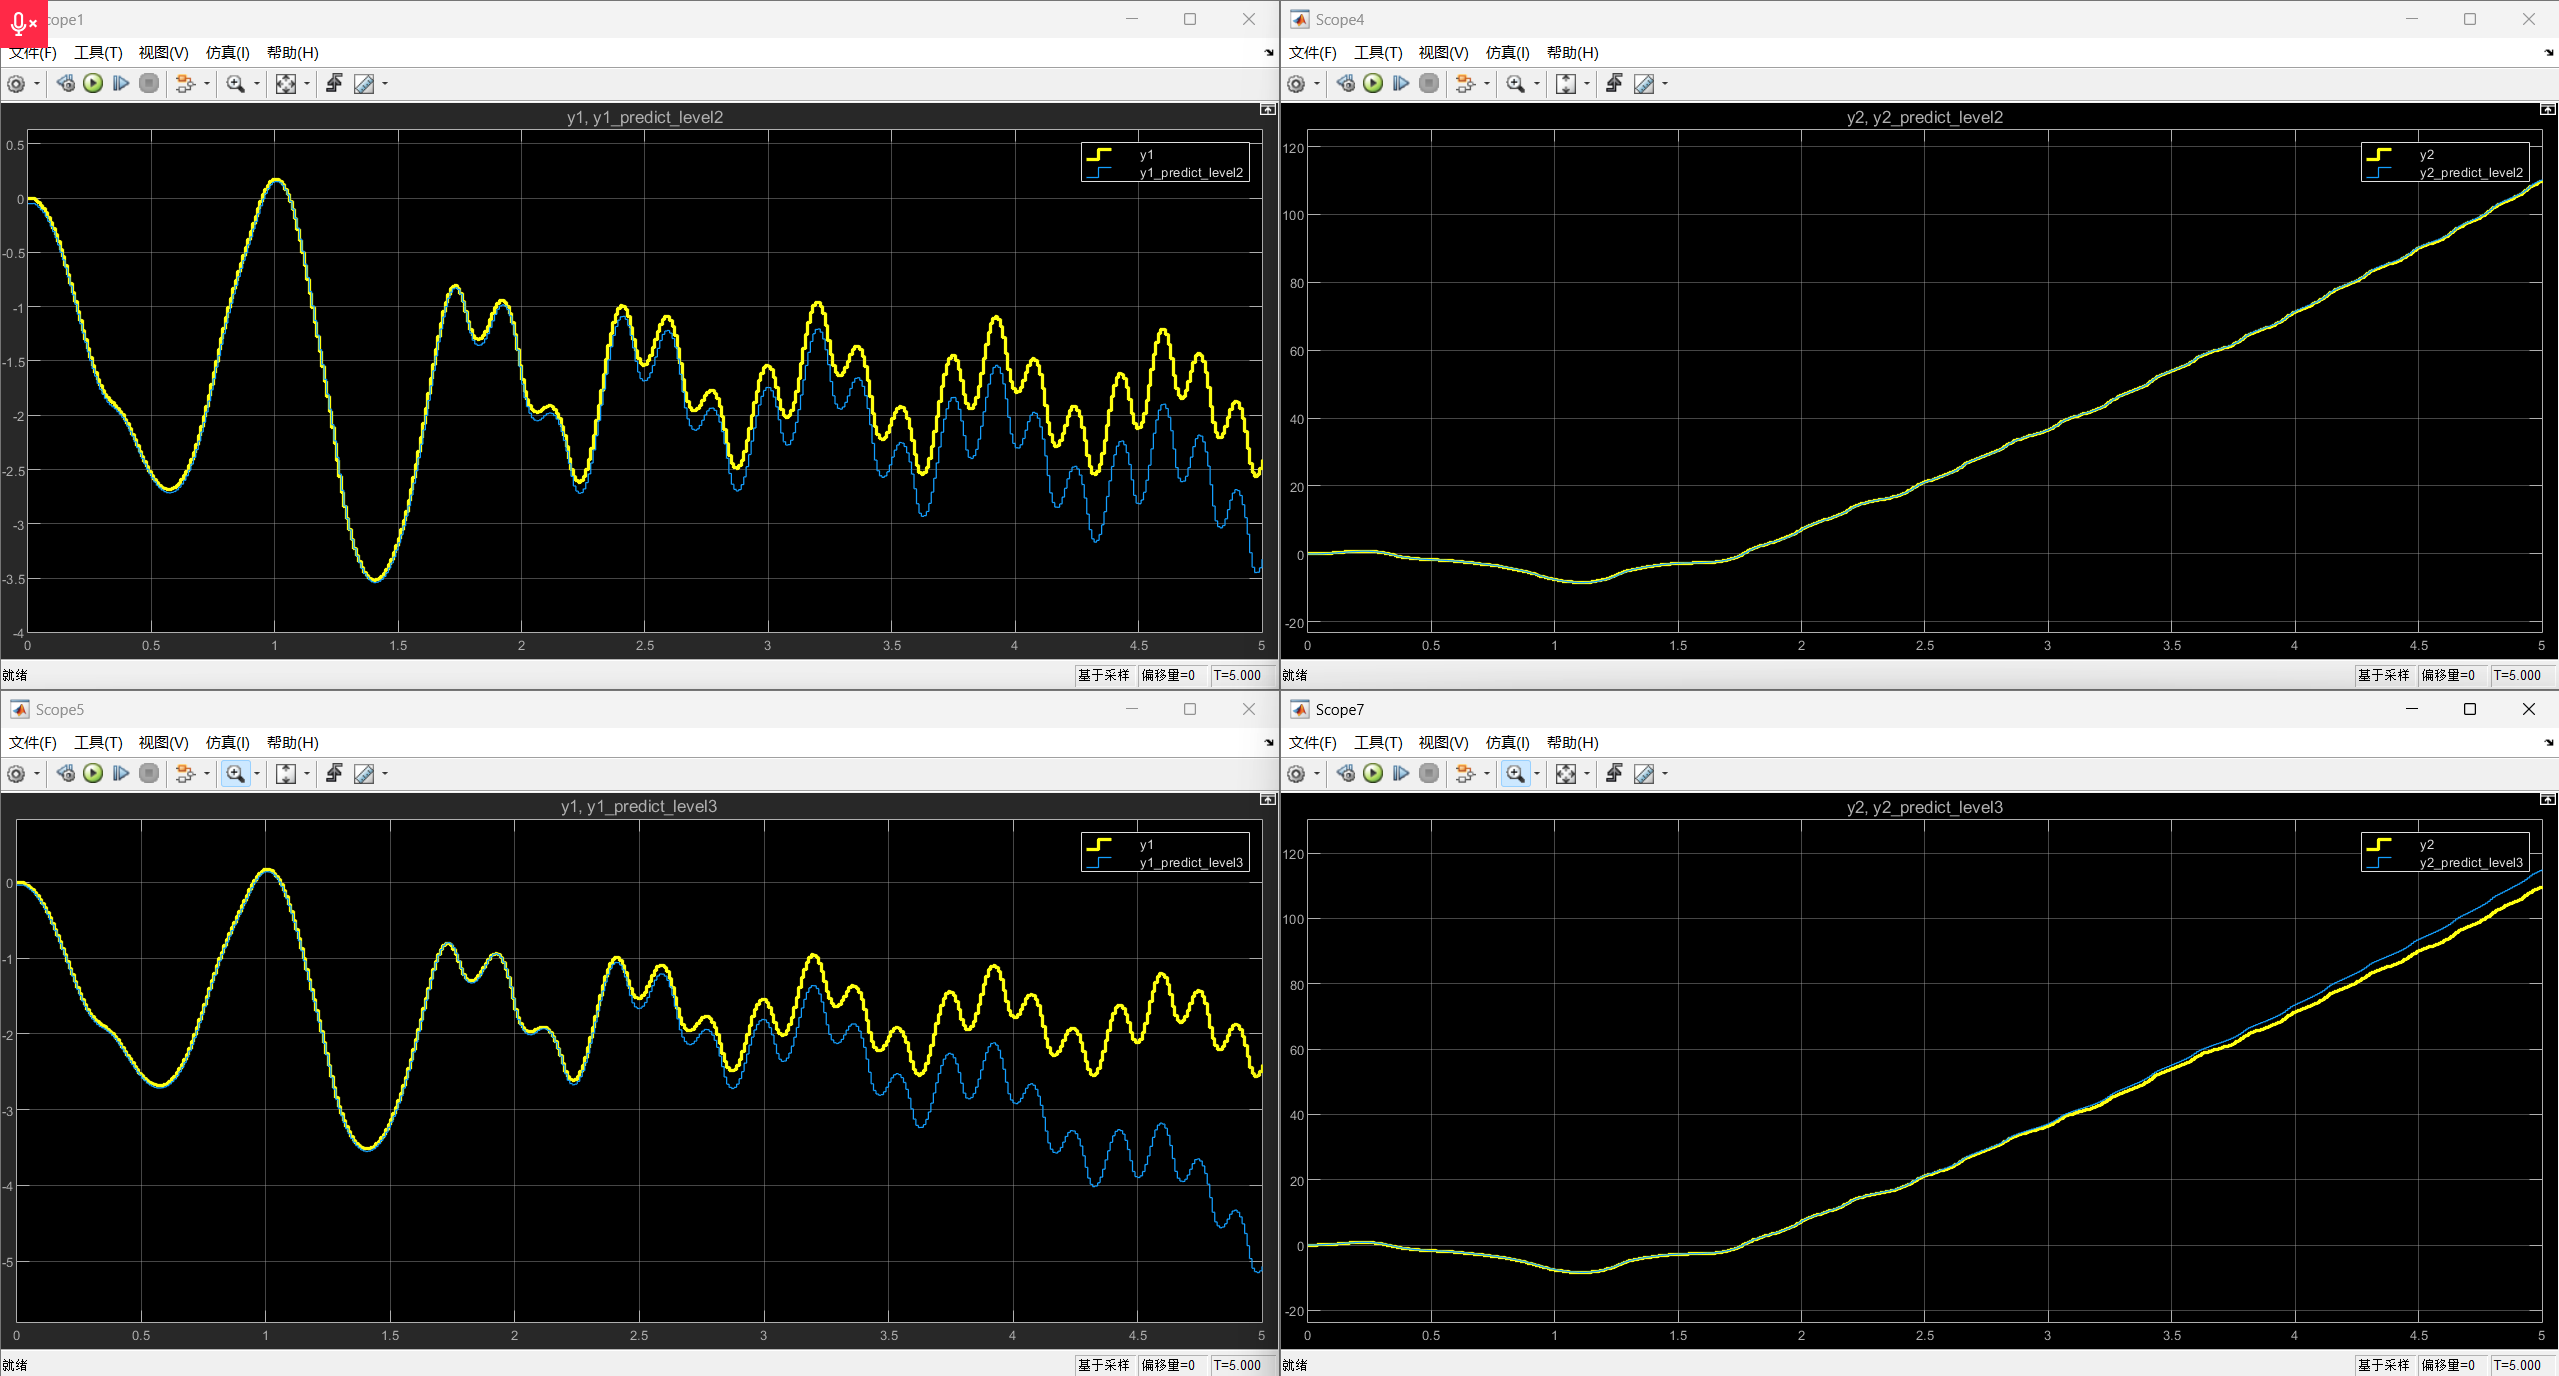
\includegraphics[width=0.7\textwidth]{figures/2024-12-24-00-25-35.png} \caption{三角输入} \label{  }\end{figure}


\begin{figure}[htbp] \centering 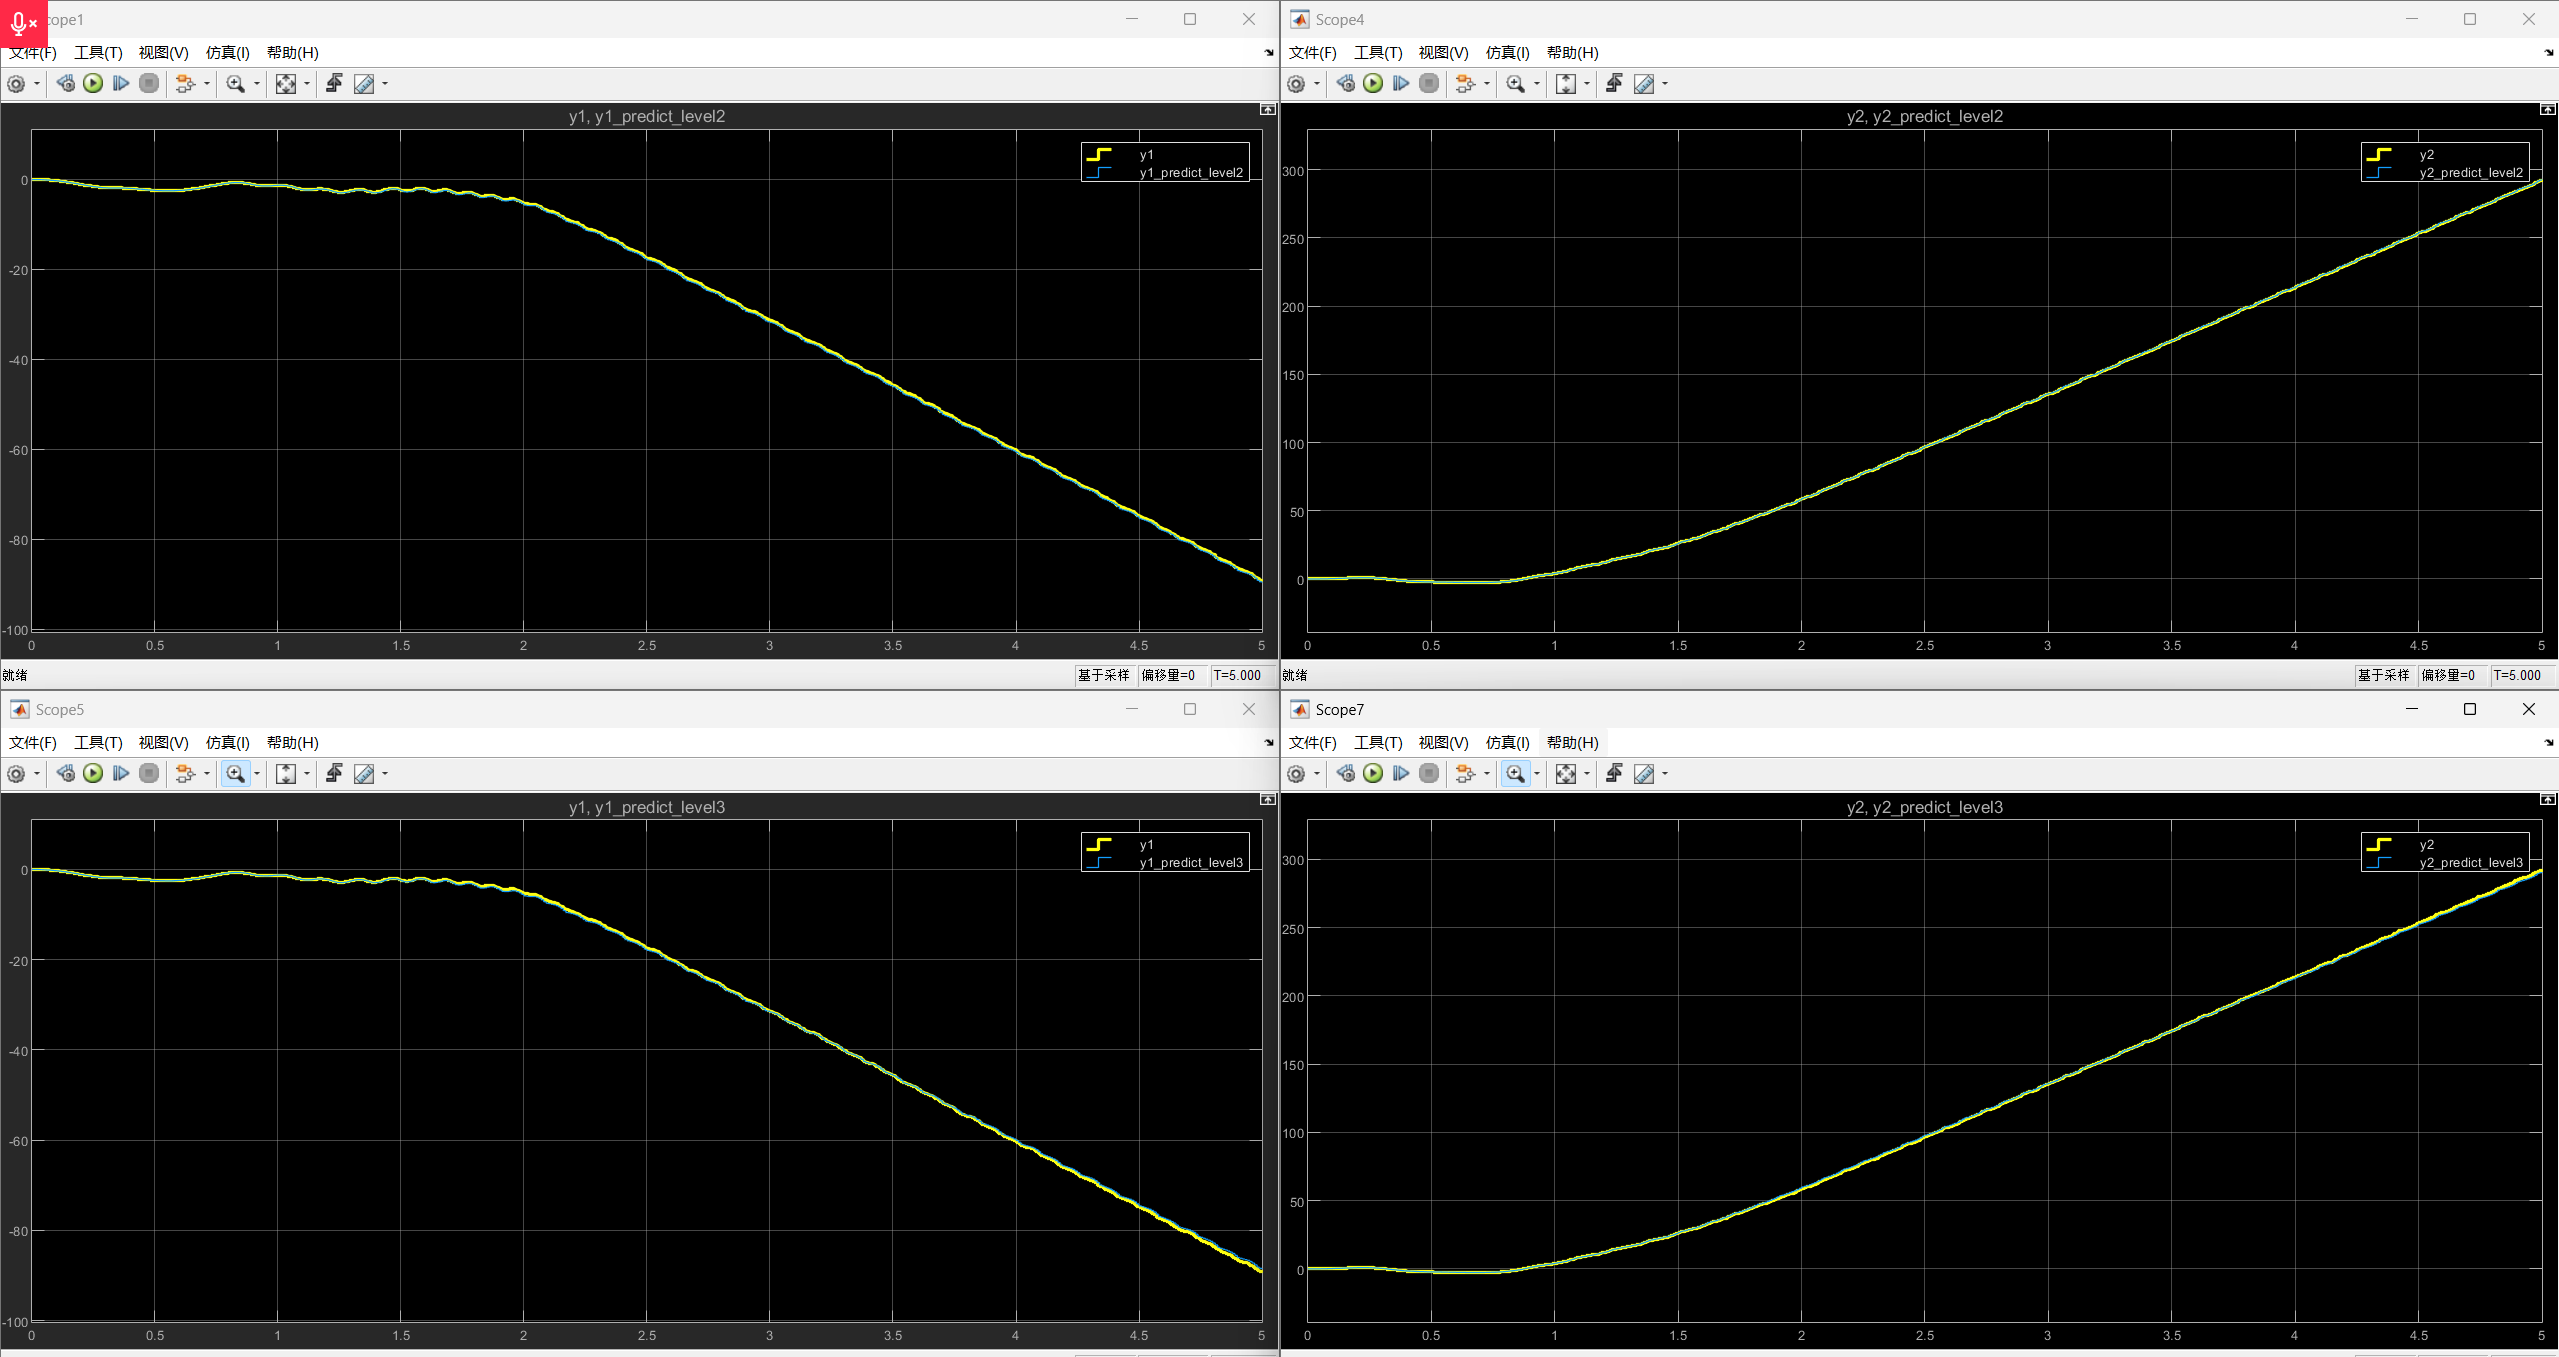
\includegraphics[width=0.7\textwidth]{figures/2024-12-24-00-26-26.png} \caption{阶跃输入} \label{  }\end{figure}


\newpage
\subsection{不同隐藏层数量(15,30)下的效果对比}

可以发现,隐藏层越多,阶数越高,训练的时间就越长

\begin{figure}[htbp] \centering 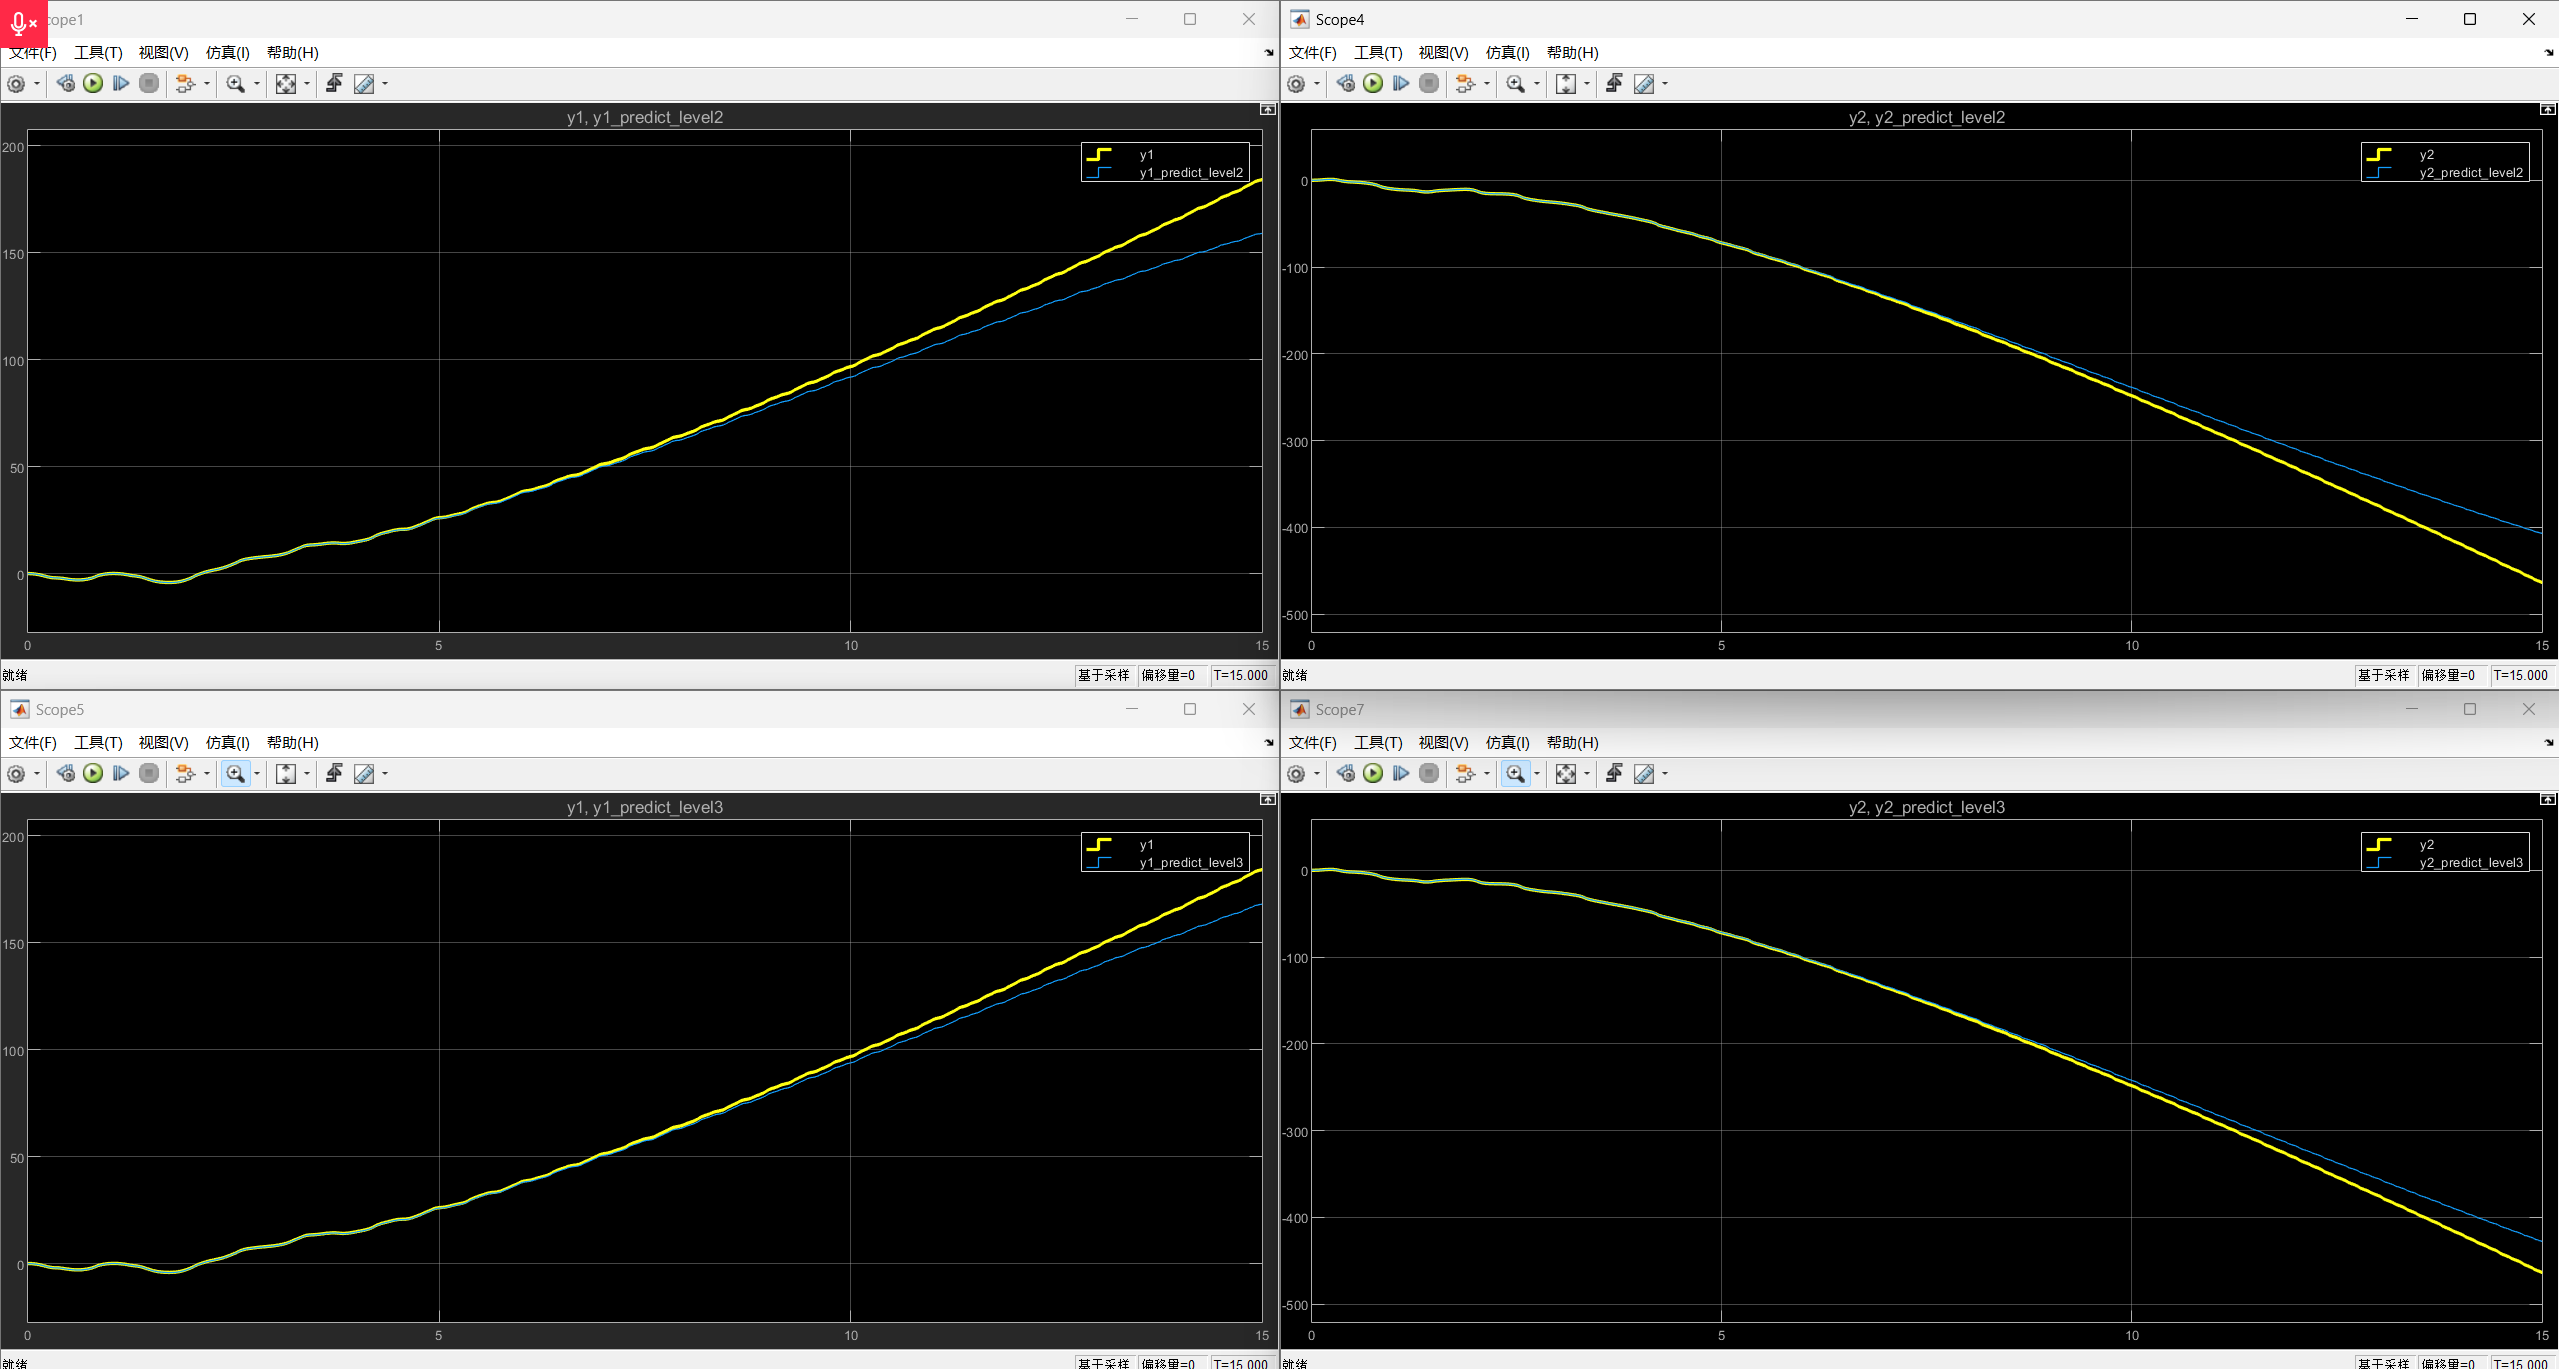
\includegraphics[width=0.7\textwidth]{figures/2024-12-24-00-39-53.png} \caption{隐藏层30 正弦输入} \label{  }\end{figure}


\begin{figure}[htbp] \centering 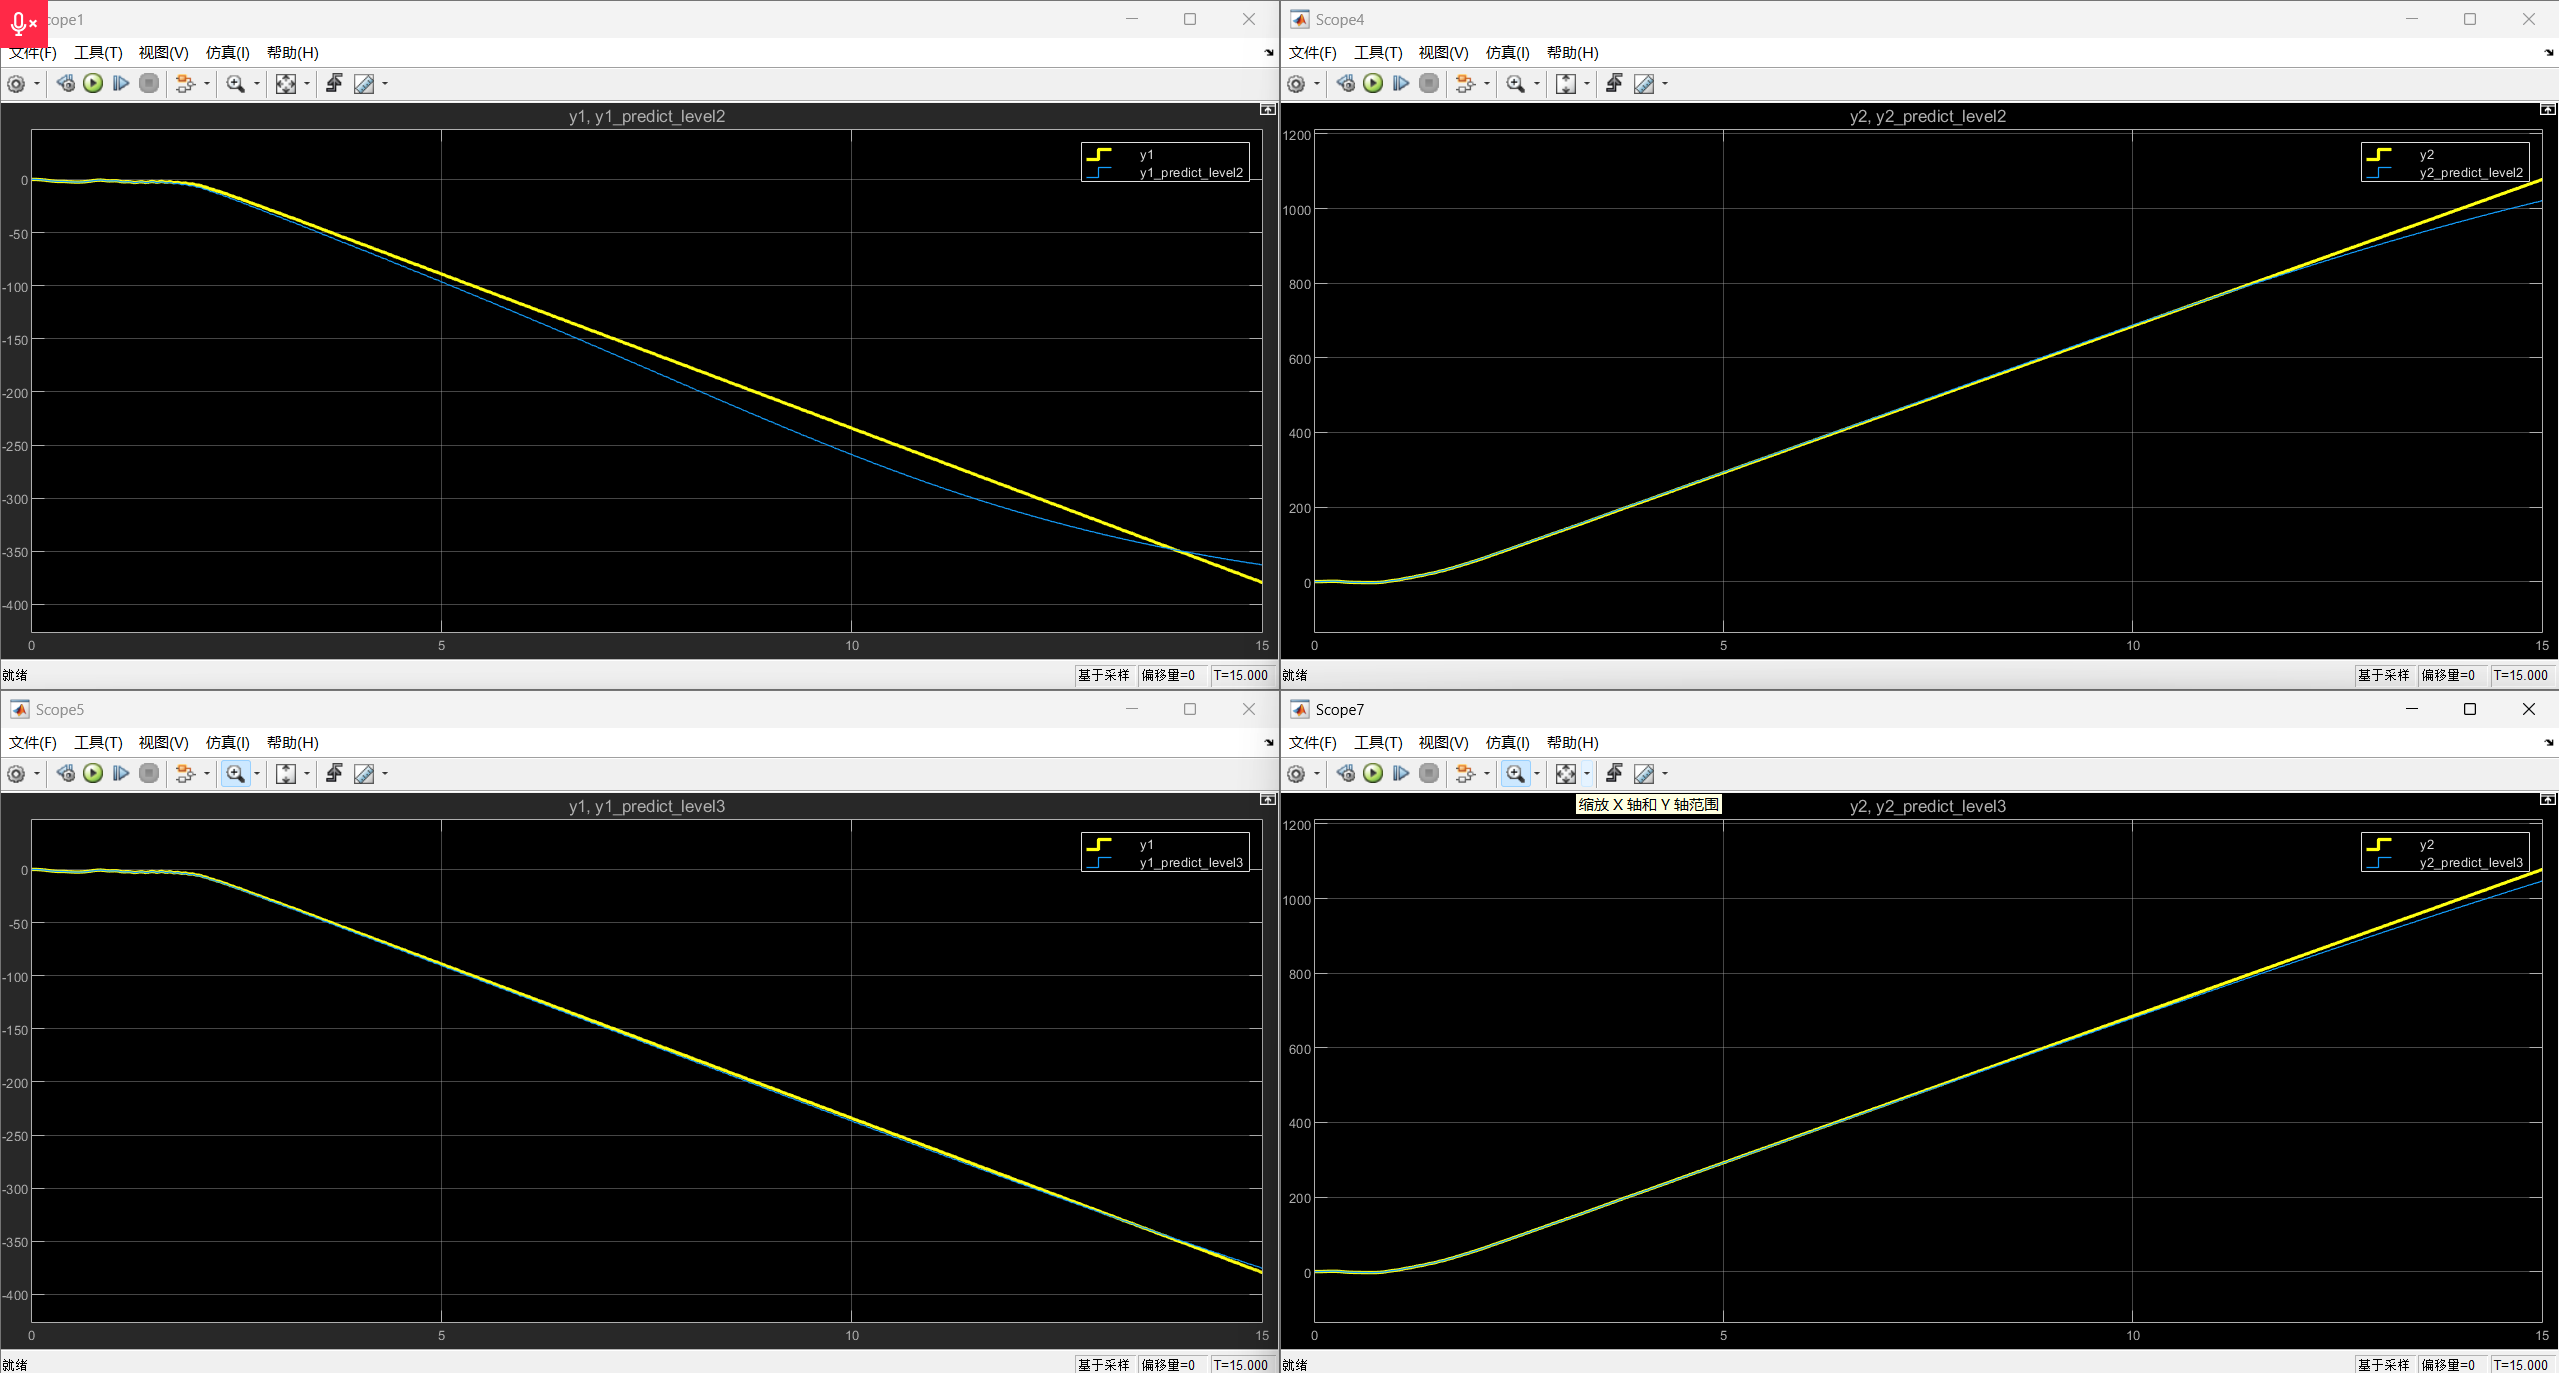
\includegraphics[width=0.7\textwidth]{figures/2024-12-24-00-40-59.png} \caption{隐藏层30 阶跃输入} \label{  }\end{figure}

这里可以发现,隐藏层30的模型,在正弦输入下,效果不如隐藏层15的模型
但是3阶模型的效果要比二阶模型的效果要好

\subsection{小结}
因为这次作业对模型精度的要求并不高,所以对于每一种情况,并没有做参数调优

总结下来,我发现有以下规律



\begin{itemize}
    \item 时间长一点的模型,效果一般不错
    \item 隐藏层数量稍微多一点,效果越好,但也不是越多越好
    \item 调整隐藏层对于结果的影响并不是特别大
    \item 如果测试和训练的信号相差比较大的话,一般会出现跑飞的情况
    \item 训练太久会出现过拟合的情况,泛化性能反而下降
\end{itemize}

\clearpage
\section{实验探索——使用pytorch训练模型并导入matlab}

由于这个学期还学习了人工智能和机器学习课程,对python的pytorch库有一定的了解

所以就想试一下matlab和simulink是否可以使用pytorch训练的模型进行预测

\subsection{环境配置和测试}

首先下载Deep Learning Toolbox Converter for ONNX Model Format


% \begin{figure}[htbp]
%     \centering
%     \includegraphics[width=0.8\textwidth]{20241223223234.png}
%     \caption{下载ONNX转换工具}
% \end{figure}

\href{https://ww2.mathworks.cn/help/deeplearning/ref/onnxmodelpredict.html}{ONNX Model Predict}

1. 使用pytorch训练之后,导出onnx模型

\begin{lstlisting}[language=Python,caption=使用pytorch训练模型]
# 使用pytorch训练模型
import torch
import torch.nn as nn
import torch.optim as optim
from torch.utils.data import DataLoader, TensorDataset
import scipy.io as sio

# Step 1: Load Data
data = sio.loadmat('data_level2.mat')
inputs = torch.tensor(data['features_level2'], dtype=torch.float32)
targets = torch.tensor(data['labels_level2'], dtype=torch.float32)

# Step 2: Prepare Dataset and DataLoader
dataset = TensorDataset(inputs, targets)
dataloader = DataLoader(dataset, batch_size=32, shuffle=True)

# Step 3: Define the Model
class RoboticArmNet(nn.Module):
    def __init__(self, input_size, output_size):
        super(RoboticArmNet, self).__init__()
        # 简单的三层网络结构
        self.net = nn.Sequential(
            nn.Linear(input_size, 32),
            nn.ReLU(),
            nn.Linear(32, 16),
            nn.ReLU(),
            nn.Linear(16, output_size)
        )
        
        # 初始化权重
        for m in self.modules():
            if isinstance(m, nn.Linear):
                nn.init.xavier_normal_(m.weight)
                nn.init.zeros_(m.bias)

    def forward(self, x):
        return self.net(x)

# Initialize the model
input_size = inputs.shape[1]  # 8
output_size = targets.shape[1]  # 2
print(input_size, output_size)
model = RoboticArmNet(input_size, output_size)

# Step 4: Define Loss and Optimizer
criterion = nn.MSELoss()
# 使用Adam优化器,通常收敛更快且效果更好
optimizer = optim.Adam(model.parameters(), lr=0.001)
# 学习率调度器
scheduler = optim.lr_scheduler.ReduceLROnPlateau(optimizer, mode='min', factor=0.5, patience=5)

# Step 5: 划分训练集和测试集
total_size = len(dataset)
train_size = int(0.8 * total_size)
test_size = total_size - train_size
train_dataset, test_dataset = torch.utils.data.random_split(dataset, [train_size, test_size])

train_loader = DataLoader(train_dataset, batch_size=32, shuffle=True)
test_loader = DataLoader(test_dataset, batch_size=32, shuffle=False)

# Step 6: 训练模型
epochs = 200  # 增加训练轮次
best_loss = float('inf')
for epoch in range(epochs):
    model.train()
    epoch_loss = 0
    for batch_inputs, batch_targets in train_loader:
        # 前向传播
        outputs = model(batch_inputs)
        loss = criterion(outputs, batch_targets)
        epoch_loss += loss.item()

        # 反向传播和优化
        optimizer.zero_grad()
        loss.backward()
        # 梯度裁剪,防止梯度爆炸
        torch.nn.utils.clip_grad_norm_(model.parameters(), max_norm=1.0)
        optimizer.step()
    
    avg_loss = epoch_loss / len(train_loader)
    scheduler.step(avg_loss)  # 更新学习率
    
    if avg_loss < best_loss:
        best_loss = avg_loss
        torch.save(model.state_dict(), 'best_model_level2.pth')

    if (epoch + 1) % 10 == 0:
        print(f'训练轮次 [{epoch + 1}/{epochs}], 平均损失: {avg_loss:.4f}')

# Step 7: 测试模型
model.eval()
test_loss = 0
with torch.no_grad():
    for inputs, targets in test_loader:
        outputs = model(inputs)
        test_loss += criterion(outputs, targets).item()
        
avg_test_loss = test_loss / len(test_loader)
print(f'测试集平均损失: {avg_test_loss:.4f}')

# 计算关节角度误差(以度为单位)
model.eval()
total_angle_error = 0
with torch.no_grad():
    for inputs, targets in test_loader:
        outputs = model(inputs)
        # 假设输出是弧度,转换为角度
        angle_error = torch.abs(outputs - targets) * 180 / 3.14159
        total_angle_error += torch.mean(angle_error).item()

avg_angle_error = total_angle_error / len(test_loader)
print(f'平均关节角度误差: {avg_angle_error:.2f}度')

# Step 8: 保存模型
torch.save(model.state_dict(), 'model_level2.pth')
torch.onnx.export(model, torch.randn(1, input_size), 'model_level2.onnx', input_names=['input'], output_names=['output'])
\end{lstlisting}



2. 在matlab中使用onnxmodelpredict函数进行预测(验证可行性)

\begin{lstlisting}[language=Matlab,caption=使用onnxmodelpredict函数进行预测]
model = importONNXNetwork('model.onnx', ...
    'OutputLayerType', 'regression', ...
    'InputDataFormats', 'BC');  % B=batch size, C=channels

% 我训练的模型输入8维,输出2维
u = [1.1; 1.1; 1.1; 1.1; 2.2; 2.2; 2.2; 2.2];
u = reshape(u, [1, 8]); % 将输入调整为 [1, 8]
y = predict(model, u);
disp('预测输出:');
disp(y);
\end{lstlisting}

3. 在simulink中使用matlab function进行预测

\subsection{遇到的问题和解决方案}

\textbf{问题1:} \texttt{Class mismatch for variable '<output of predict>'. Expected 'double', Actual 'single'.}

需要强制类型转换一下:
\begin{lstlisting}[language=Matlab]
y_single = predict(model, u);  % 返回的预测结果是 single 类型
y = double(y_single);  % 将结果转换为 double 类型
\end{lstlisting}

\textbf{问题2:} \texttt{MATLAB Function 'xxx' not supported for code generation.}

参考: \href{https://blog.csdn.net/qq_38146340/article/details/118675853}{simulink函数输出中不能为mxarray}

simulink代码生成的过程中,有些函数不支持内部代码生成,需要将其定义为外部函数,使用\texttt{coder.extrinsic}声明:
\begin{lstlisting}[language=Matlab]
coder.extrinsic('name_of_the_function');
\end{lstlisting}

\textbf{提示:} 防止重复导入模型的方法

为了防止matlab function每次调用时都导入一遍模型,使用\texttt{persistent}关键字声明模型,这样可以大大提高运行速度:

\begin{lstlisting}[language=Matlab]
function y = predictWithONNX(u)
    persistent model; 
    coder.extrinsic('importONNXNetwork'); % 声明外部函数
    if isempty(model)
        % 仅当模型未加载时加载 ONNX 模型,防止重复加载消耗时间
        model = importONNXNetwork('model_level2.onnx', ...
            'OutputLayerType', 'regression', ...
            'InputDataFormats', 'BC');  % B=batch size, C=channels
    end

    y = zeros(1, 2);    % 初始化输出并调整输入格式
    u = reshape(u, [1, 8]);  % 确保输入尺寸匹配
    coder.extrinsic('predict');
    y_single = predict(model, u);  % 返回的预测结果是 single 类型
    y = double(y_single);  % 将结果转换为 double 类型
end
\end{lstlisting}

\subsection{实验结果}

\begin{figure}[htbp] \centering 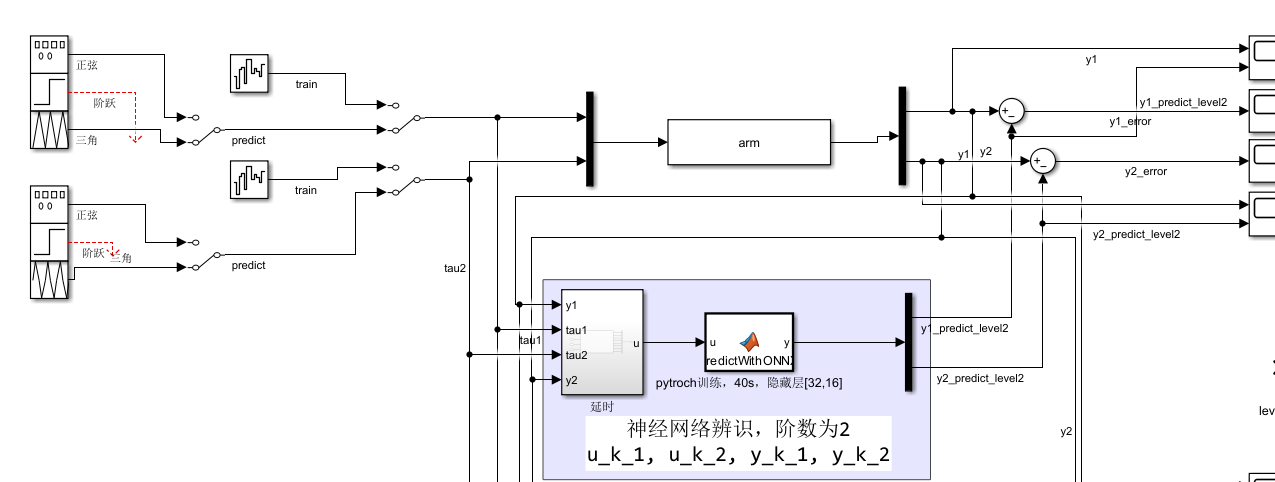
\includegraphics[width=\textwidth]{figures/2024-12-23-23-20-29.png} \caption{使用matlab function 加载模型} \label{  }\end{figure}

切换到predict模式,发现正弦输入不太能跟住

\begin{figure}[htbp] 
\centering 
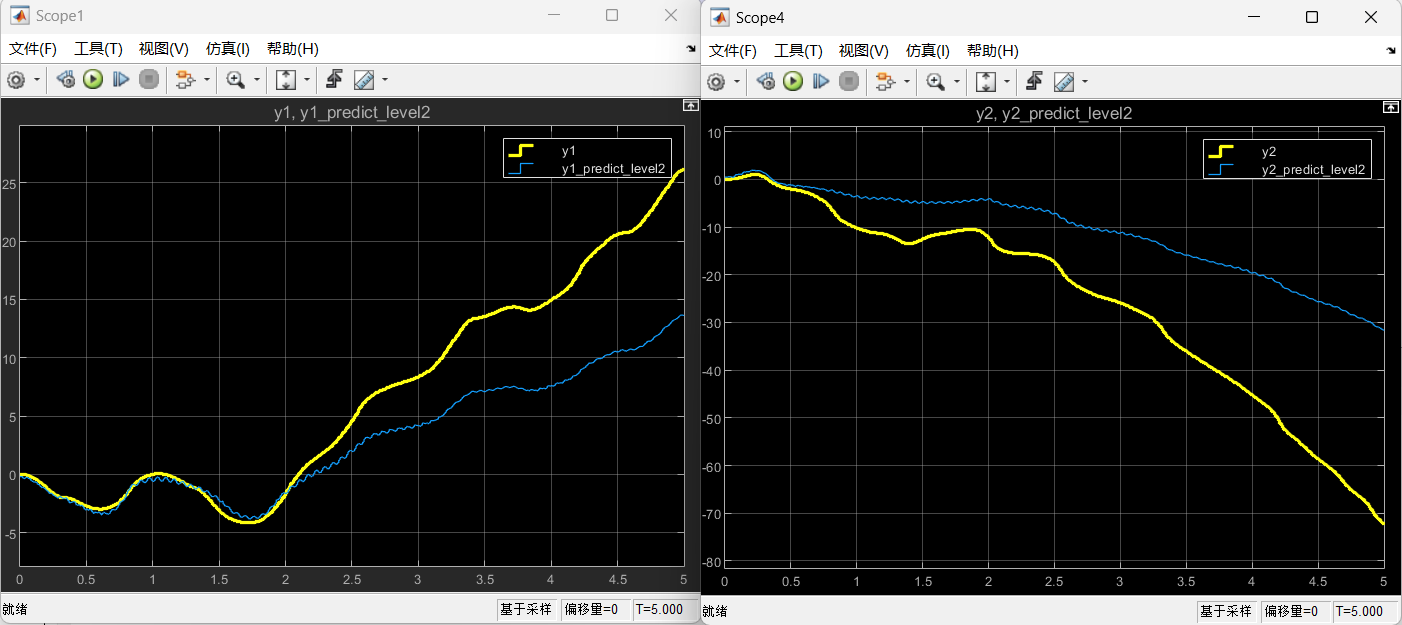
\includegraphics[width=0.9\textwidth]{figures/2024-12-23-23-13-26.png} \caption{正弦输入} \label{  }\end{figure}


阶跃输入跟的还是不错的

\begin{figure}[htbp] \centering 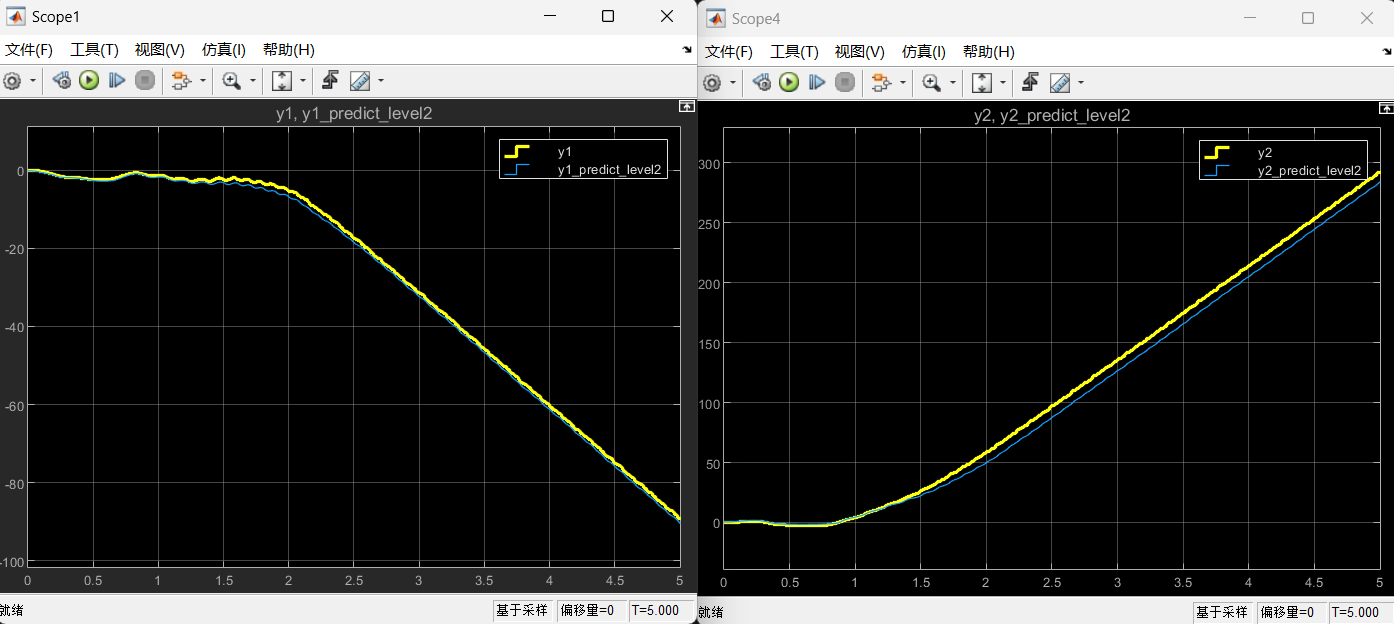
\includegraphics[width=0.7\textwidth]{figures/2024-12-23-23-14-27.png} \caption{阶跃输入} \label{  }\end{figure}

三角输入稳定性也不太好
\begin{figure}[htbp] \centering 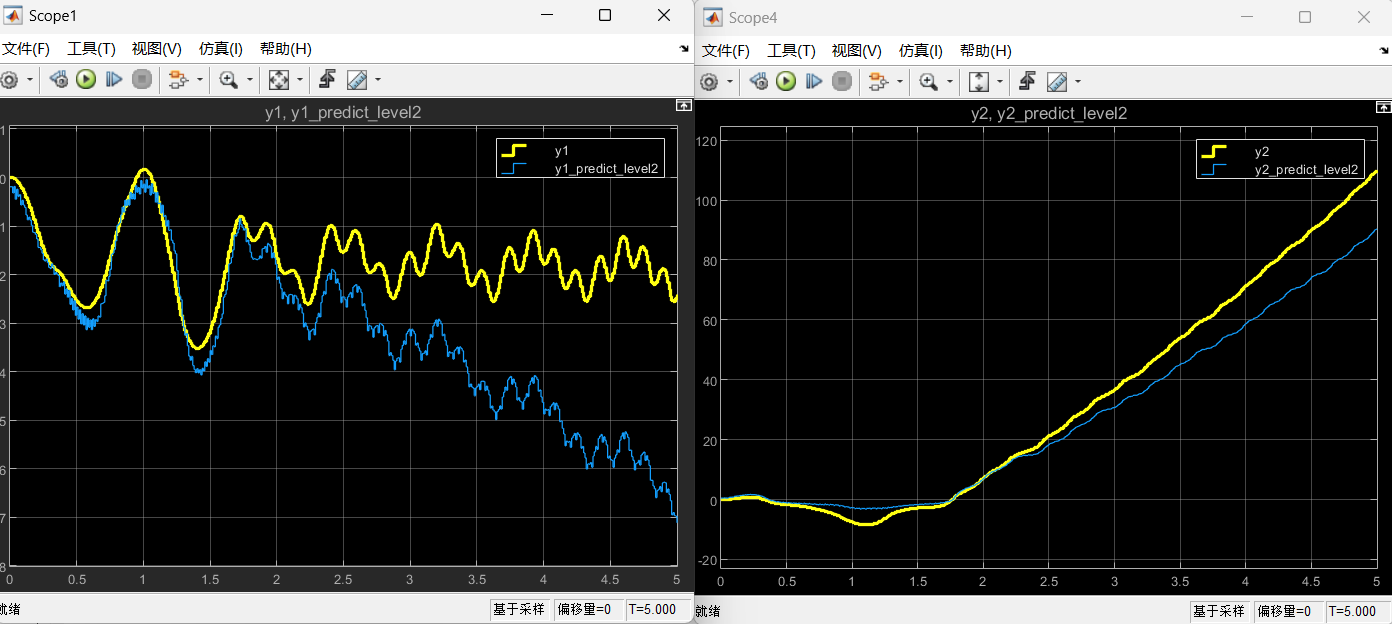
\includegraphics[width=0.7\textwidth]{figures/2024-12-23-23-15-31.png} \caption{三角输入} \label{  }\end{figure}


由于这种方法最初只是为了验证matlab使用pytorch训练的模型进行预测的可行性,所以pytorch训练的代码中模型的选择和训练参数没有做太多优化和调节,所以最后的效果并不是太理想。

如果后续优化的话,可以重点从模型的结果和超参数的调节入手。

通过各种资料解决了环境配置和代码的问题,最后成功实现了这个功能,还是挺有成就感的。


\clearpage
\appendix
\section{附录1:源程序代码}

\dirtree{%
.1 .
.2 README.md.
.2 report.
.3 ref.bib.
.3 thesis.tex.
.3 figures.
.2 src.
.3 arm.m \dotfill 2-DOF机械臂的simulink模型.
.3 data\_level2.mat.
.3 data\_level3.mat.
.3 model.slx \dotfill 仿真文件.
.3 train.m \dotfill 使用matlab训练模型.
.3 train\_pytorch.py \dotfill 使用pytorch训练模型.
.3 test\_pytorch.m \dotfill 使用pytorch训练的模型进行测试.
.3 model\_level2.onnx \dotfill 使用pytorch训练的模型文件.
.3 learn\_toolbox \dotfill 神经网络工具箱的学习过程以及数据文件.
.4 test\_multi.m.
.4 test\_train.m.
.4 test\_train.mat.
.4 untitled19.m.
.4 神经网络案例——辛烷值和光谱分析.xlsx.
}

\begin{lstlisting}[language=Matlab,caption=arm.m——2-DOF 机械臂的物理模型 S-function实现]
function [sys, x0, str, ts, simStateCompliance] = arm(t, x, u, flag)
    global input_data output_data time_data; % 全局变量存储数据
    switch flag
        case 0
            [sys, x0, str, ts, simStateCompliance] = mdlInitializeSizes();
        case 2
            sys = mdlUpdate(t, x, u);
        case 3
            sys = mdlOutputs(t, x, u);
        case 9
            sys = mdlTerminate();
        otherwise
            DAStudio.error('Simulink:blocks:unhandledFlag', num2str(flag));
    end
end

function [sys, x0, str, ts, simStateCompliance] = mdlInitializeSizes()
    global input_data output_data time_data;

    % 初始化全局变量
    input_data = [];
    output_data = [];
    time_data = [];

    sizes = simsizes;
    sizes.NumContStates  = 0;  % 无连续状态
    sizes.NumDiscStates  = 4; % 离散状态:[q1, q2, dq1, dq2]
    sizes.NumOutputs     = 2; % 输出:q1, q2
    sizes.NumInputs      = 2; % 输入:tau1, tau2
    sizes.DirFeedthrough = 0; % 无直接传递
    sizes.NumSampleTimes = 1; % 单一采样时间

    sys = simsizes(sizes);

    x0 = [0; 0; 0; 0]; % 初始状态:[q1, q2, dq1, dq2]
    str = [];
    ts = [0.01 0]; % 设置采样时间为 0.01 秒
    simStateCompliance = 'UnknownSimState'; % 仿真状态合规性
end

function sys = mdlUpdate(t, x, u)
    global input_data;
    input_data = [input_data; u(1), u(2)];     % 记录输入
    % 提取状态变量和输入
    q1 = x(1); q2 = x(2);       % 关节角
    dq1 = x(3); dq2 = x(4);     % 关节角速度
    tau1 = u(1); tau2 = u(2);   % 输入力矩

    % 系统参数
    h1 = 0.0308; h2 = 0.0106; h3 = 0.0095;
    h4 = 0.2086; h5 = 0.0631; g = 9.8;

    % 惯性矩阵 M(q)
    m11 = h1 + h2 + 2 * h3 * cos(q2);
    m12 = h2 + h3 * cos(q2);
    M = [m11, m12; m12, h2];

    % 科氏力和向心力矩阵 C(q, dq)
    c11 = -h3 * sin(q2) * dq2;
    c12 = -h3 * sin(q2) * (dq1 + dq2);
    c21 = h3 * sin(q2) * dq1;
    C = [c11, c12; c21, 0];

    % 重力矩阵 G(q)
    g1 = h4 * g * cos(q1) + h5 * g * cos(q1 + q2);
    g2 = h5 * g * cos(q1 + q2);
    G = [g1; g2];

    % 动力学方程求解加速度
    ddq = M \ (u - C * [dq1; dq2] - G);

    % 离散状态更新(积分)
    dt = 0.01; % 采样时间
    q1_next = q1 + dq1 * dt;
    q2_next = q2 + dq2 * dt;
    dq1_next = dq1 + ddq(1) * dt;
    dq2_next = dq2 + ddq(2) * dt;

    % 返回更新后的状态
    sys = [q1_next; q2_next; dq1_next; dq2_next];
end

function sys = mdlOutputs(t, x, u)
    global input_data output_data time_data;

    % 记录输入和输出数据
    
    output_data = [output_data; x(1:2)'];      % 记录输出
    time_data = [time_data; t];                % 记录时间

    sys = [x(1); x(2)]; % 返回输出
end

function sys = mdlTerminate()
    global input_data output_data time_data;

    % 仿真结束时保存数据到 data_level2.mat 和 data_level3.mat
    % 确保输入输出数据长度一致
    n = min(size(input_data, 1), size(output_data, 1));
    input_data = input_data(1:n, :);
    output_data = output_data(1:n, :);

    %% 二阶数据保存
    y_k_2 = output_data(1:end-2, :);  % y_k-2,从第1个样本开始到倒数第3个
    y_k_1 = output_data(2:end-1, :);  % y_k-1,从第2个样本开始到倒数第2个
    u_k_2 = input_data(1:end-2, :);   % u_k-2,从第1个样本开始到倒数第3个
    u_k_1 = input_data(2:end-1, :);   % u_k-1,从第2个样本开始到倒数第2个
    y_k = output_data(3:end, :);      % 输出向量,从第3个样本开始

    % 拼接特征矩阵和标签(二阶)
    features_level2 = [u_k_1, u_k_2, y_k_1, y_k_2];
    labels_level2 = y_k;

    save('data_level2.mat', 'features_level2', 'labels_level2', 'time_data');

    %% 三阶数据保存
    y_k_3 = output_data(1:end-3, :);  % y_k-3,从第1个样本开始到倒数第4个
    y_k_2 = output_data(2:end-2, :);  % y_k-2,从第2个样本开始到倒数第3个
    y_k_1 = output_data(3:end-1, :);  % y_k-1,从第3个样本开始到倒数第2个
    u_k_3 = input_data(1:end-3, :);   % u_k-3,从第1个样本开始到倒数第4个
    u_k_2 = input_data(2:end-2, :);   % u_k-2,从第2个样本开始到倒数第3个
    u_k_1 = input_data(3:end-1, :);   % u_k-1,从第3个样本开始到倒数第2个
    y_k = output_data(4:end, :);      % 输出向量,从第4个样本开始

    % 拼接特征矩阵和标签(三阶)
    features_level3 = [u_k_1, u_k_2, u_k_3, y_k_1, y_k_2, y_k_3];
    labels_level3 = y_k;

    save('data_level3.mat', 'features_level3', 'labels_level3', 'time_data');


    sys = []; % 终止函数无返回值
end
    
\end{lstlisting}


\begin{lstlisting}[language=Python,caption=test\_pytorch.m——验证加载pytorch训练模型的可行性]
% 验证加载pytorch训练模型的可行性

% 加载 ONNX 模型
% 添加 InputDataFormats 参数来指定输入格式
model = importONNXNetwork('model_level2.onnx', ...
    'OutputLayerType', 'regression', ...
    'InputDataFormats', 'BC');  % B=batch size, C=channels

% 示例输入
u = [1.1; 1.1; 1.1; 1.1; 2.2; 2.2; 2.2; 2.2];
u = reshape(u, [1, 8]); % 将输入调整为 [1, 8]

% 预测
y = predict(model, u);

% 显示预测结果
disp('预测输出:');
disp(y);
\end{lstlisting}

\begin{lstlisting}[language=Matlab,caption=train.m——使用matlab训练模型的脚本]
function train(level)
    % 输入:
    % level - 指定数据级别,1表示level2,2表示level3等

    % 根据level加载相应的数据文件
    if level == 2
        dataFile = 'data_level2.mat';
    elseif level == 3
        dataFile = 'data_level3.mat';
    else
        error('Unsupported level: %d. Only level 2 and level 3 are supported.', level);
    end
    
    % 加载数据
    load(dataFile);  % 导入数据

    % 根据 level 动态选择相应的数据变量
    if level == 2
        x = features_level2';  % 转置为符合网络输入格式
        t = labels_level2';  % 转置为符合网络目标格式
    elseif level == 3
        x = features_level3';  % 转置为符合网络输入格式
        t = labels_level3';  % 转置为符合网络目标格式
    end

    % 选择训练函数
    trainFcn = 'trainlm';  % Levenberg-Marquardt 反向传播

    % 创建拟合网络
    hiddenLayerSize = 30;
    net = fitnet(hiddenLayerSize, trainFcn);

    % 输入输出的预处理函数
    net.input.processFcns = {'removeconstantrows', 'mapminmax'};
    net.output.processFcns = {'removeconstantrows', 'mapminmax'};

    % 设置数据的划分方式
    net.divideFcn = 'dividerand';  % 随机划分数据
    net.divideMode = 'sample';  % 划分所有样本
    net.divideParam.trainRatio = 70/100;
    net.divideParam.valRatio = 15/100;
    net.divideParam.testRatio = 15/100;

    % 选择性能函数
    net.performFcn = 'mse';  % 均方误差

    % 选择绘图函数
    net.plotFcns = {'plotperform', 'plottrainstate', 'ploterrhist', ...
        'plotregression', 'plotfit'};

    % 训练网络
    [net, tr] = train(net, x, t);

    % 测试网络
    y = net(x);
    e = gsubtract(t, y);
    performance = perform(net, t, y);

    % 重新计算训练、验证和测试性能
    trainTargets = t .* tr.trainMask{1};
    valTargets = t .* tr.valMask{1};
    testTargets = t .* tr.testMask{1};
    trainPerformance = perform(net, trainTargets, y);
    valPerformance = perform(net, valTargets, y);
    testPerformance = perform(net, testTargets, y);

    % 确保 figures 文件夹存在
%     if ~exist('figures', 'dir')
%         mkdir('figures');
%     end

    % 绘制并保存训练性能图
%     figure, plotperform(tr);
%     saveas(gcf, ['figures/plotperform_level' num2str(level) '.fig']);  % 保存为 .fig 文件

    % 绘制并保存训练状态图
%     figure, plottrainstate(tr);
%     saveas(gcf, ['figures/plottrainstate_level' num2str(level) '.fig']);  % 保存为 .fig 文件

    % 绘制并保存误差直方图
%     figure, ploterrhist(e);
%     saveas(gcf, ['figures/ploterrhist_level' num2str(level) '.fig']);  % 保存为 .fig 文件

    % 绘制并保存回归图
%     figure, plotregression(t, y);
%     saveas(gcf, ['figures/plotregression_level' num2str(level) '.fig']);  % 保存为 .fig 文件

    % 绘制并保存拟合图
%     figure, plotfit(net, x, t);
%     saveas(gcf, ['figures/plotfit_level' num2str(level) '.fig']);  % 保存为 .fig 文件

    % 保存模型
%     modelFile = ['model_level' num2str(level) '.mat'];
%     save(modelFile, 'net');  % 保存神经网络模型
    gensim(net);
end
\end{lstlisting}

\section{附录2:版本更新记录}


\begin{table}[htbp]
\centering
\caption{版本更新记录}
\begin{tabular}{|c|l|}
\hline
时间 & 更新内容 \\
\hline
12.23上午 & 完成机械臂模型的s-function编写,实现数据采集功能 \\
\hline
12.23下午 & 完成神经网络工具箱的学习和使用,编写训练脚本 \\
\hline
12.23晚上 & 实现pytorch模型训练并导入matlab的功能 \\
\hline
12.24上午 & 完成不同参数下的模型训练和测试 \\
\hline
12.24下午 & 完成实验报告的撰写和整理 \\
\hline
\end{tabular}
\end{table}

\reference
\end{document}
